% 1977 年河北卷第 7 题：圆内直径与外部相交线
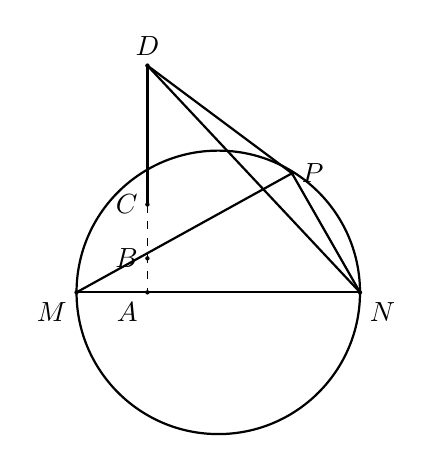
\begin{tikzpicture}[scale=0.72,>=stealth]
  \coordinate (M) at (0,0);
  \coordinate (N) at (5,0);
  \coordinate (O) at (2.5,0);
  \coordinate (P) at (3.8,2.1);
  \coordinate (C) at (1.25,1.55);
  \coordinate (D) at (1.25,4.0);
  \coordinate (A) at (1.25,0);
  \coordinate (B) at (1.25,0.6);
  \draw[thick] (M) arc (180:540:2.5);
  \draw[thick] (M)--(N);
  \draw[thick] (P)--(M) (P)--(N);
  \draw[thick] (D)--(P);
  \draw[thick] (D)--(C);
  \draw[thick] (D)--(N);
  \draw[dashed] (C)--(A);
  \fill (M) circle (1.1pt) node[below left] {$M$};
  \fill (N) circle (1.1pt) node[below right] {$N$};
  \fill (P) circle (1.1pt) node[right] {$P$};
  \fill (C) circle (1.1pt) node[left] {$C$};
  \fill (D) circle (1.1pt) node[above] {$D$};
  \fill (A) circle (1.1pt) node[below left] {$A$};
  \fill (B) circle (1.1pt) node[left] {$B$};
\end{tikzpicture}
